\documentclass[12pt, twoside]{article}
\input{../preamble}

\fancyhead[LO]{La Scuola d'Italia / Dr.\ Huson / IB Math \\* 3 June 2026}
\fancyhead[RO]{\fbox{\begin{minipage}{6cm}\footnotesize First \& Last name:\\[0.5cm]\end{minipage}}}
\fancyfoot[C]{\thepage}

\begin{document}

\subsubsection*{8.8 Classwork: Transformations and Composition}

%================================================================
%--- Part A: vocabulary / proper terms (fill-in-the-blank) ---
%================================================================
\noindent\textbf{\large Part A --- The language of transformations}

\medskip
\noindent A \emph{full} description names three things: the \textbf{type}, the
\textbf{direction}, and the \textbf{amount}.

\medskip
\noindent\fbox{\parbox{0.94\textwidth}{\centering \textbf{Word bank:}\quad
translate (shift, slide) \ \textbullet\ \ stretch (dilate, scale) \ \textbullet\ \
reflect \ \textbullet\ \ vertical \ \textbullet\ \ horizontal \ \textbullet\ \
scale factor \ \textbullet\ \ up \ \textbullet\ \ down \ \textbullet\ \ left \ \textbullet\ \ right}}

\medskip
\noindent\textbf{A1.\quad Fill in each blank with a word from the bank.}
\begin{enumerate}[itemsep=0.30cm, label=(\alph*)]
  \item A \underline{\hspace{3cm}} slides every point the same distance in the same direction.
  \item To describe a horizontal translation fully, give the number of units \emph{and} state \underline{\hspace{2.3cm}} or \underline{\hspace{2.3cm}}.
  \item A vertical \underline{\hspace{2.8cm}} with \underline{\hspace{2.8cm}} $2$ doubles every $y$-coordinate.
  \item Multiplying every output by a number is also called a \underline{\hspace{3cm}} (another word for stretch).
  \item In $y = \dfrac{a}{x} + k$, the $+k$ produces a vertical \underline{\hspace{3cm}}.
  \item The vague word ``\underline{\hspace{2.5cm}}'' does \emph{not} count as a description --- use translate, shift, or slide instead.
\end{enumerate}

\medskip
\noindent\textbf{A2.\quad The graph of $y=\dfrac1x$ is changed to $y=\dfrac1x+4$. Circle every
description that earns full credit; cross out those that do not.}
\begin{enumerate}[itemsep=0.18cm, label=(\alph*)]
  \item move up 4
  \item translate $4$ up
  \item shift $4$ in the positive $y$-direction
  \item $+4$
  \item slide vertically $4$
\end{enumerate}
\emph{A full description needs a proper word and (for horizontal moves) an explicit
direction; bare symbols do not count.}

\medskip
\noindent\textbf{A3.\quad Draw a line matching each term to an equivalent term.}
\begin{center}
\begin{tabular}{l@{\hspace{3cm}}l}
translate & dilate \\[0.25cm]
stretch   & flip \\[0.25cm]
reflect   & slide \\
\end{tabular}
\end{center}

\newpage

%================================================================
%--- Part B: describe fully, in words ---
%================================================================
\noindent\textbf{\large Part B --- Describe the transformations}

\medskip
\noindent For each function the parent graph is $y=\dfrac1x$. \textbf{Describe fully,
in words}, the sequence of transformations, and write the equations of the two
asymptotes.

\begin{enumerate}[itemsep=0.1cm, label=\arabic*.]
  \item $f(x)=\dfrac{1}{x-2}+3$ \vfill
  \item $f(x)=\dfrac{3}{x}-1$ \vfill
  \item $f(x)=-\dfrac{1}{x}$ \hfill \emph{(this one includes a reflection)} \vfill
  \item $f(x)=\dfrac{2}{x+4}$ \vfill
\end{enumerate}

\newpage

%================================================================
%--- Part C: graphing on sketch grids ---
%================================================================
\noindent\textbf{\large Part C --- Sketch the transformed graph}

\medskip
\noindent Sketch each graph on its grid. Draw the asymptotes (or axis of symmetry)
as \textbf{dashed} lines and label them, then plot at least two points.

\medskip
\noindent\textbf{1.}\quad $y=\dfrac{1}{x-2}+1$
\begin{center}
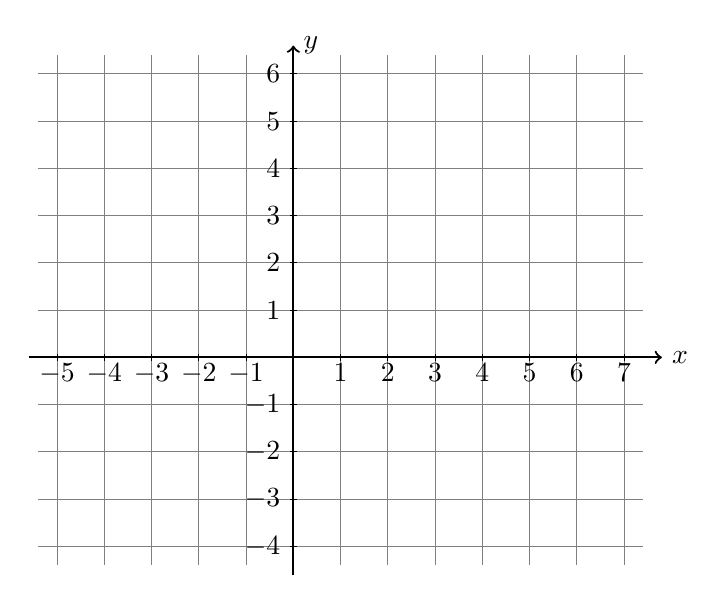
\begin{tikzpicture}[scale=0.6]
  \draw [thin, color=gray, step=1.0cm] (-5.4,-4.4) grid (7.4,6.4);
  \foreach \x in {-5,-4,-3,-2,-1,1,2,3,4,5,6,7} \draw[shift={(\x,0)}] (0pt,-2pt)--(0pt,2pt) node[below] {$\x$};
  \foreach \y in {-4,-3,-2,-1,1,2,3,4,5,6} \draw[shift={(0,\y)}] (2pt,0pt)--(-2pt,0pt) node[left] {$\y$};
  \draw [thick, ->] (-5.6,0) -- (7.8,0) node [right] {$x$};
  \draw [thick, ->] (0,-4.6) -- (0,6.6) node [right] {$y$};
\end{tikzpicture}
\end{center}

\noindent\textbf{2.}\quad $y=-(x+1)^2+4$ \quad \emph{(a transformed parabola)}
\begin{center}
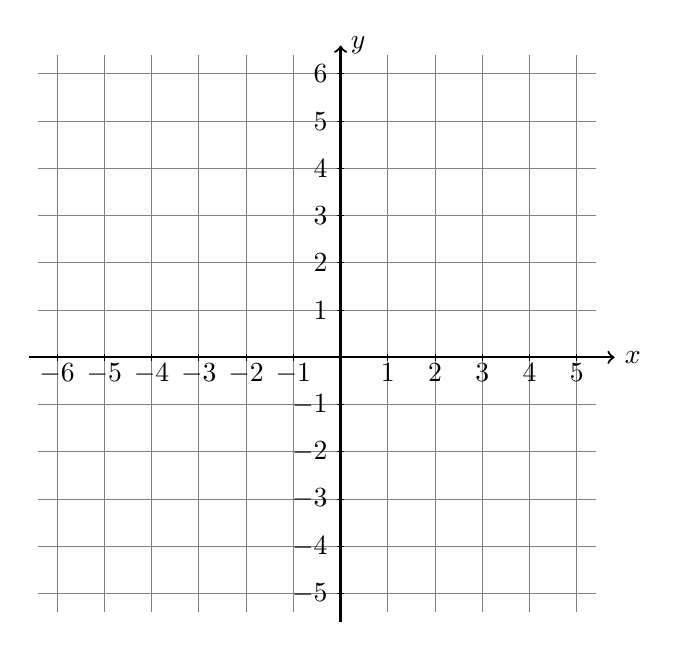
\begin{tikzpicture}[scale=0.6]
  \draw [thin, color=gray, step=1.0cm] (-6.4,-5.4) grid (5.4,6.4);
  \foreach \x in {-6,-5,-4,-3,-2,-1,1,2,3,4,5} \draw[shift={(\x,0)}] (0pt,-2pt)--(0pt,2pt) node[below] {$\x$};
  \foreach \y in {-5,-4,-3,-2,-1,1,2,3,4,5,6} \draw[shift={(0,\y)}] (2pt,0pt)--(-2pt,0pt) node[left] {$\y$};
  \draw [thick, ->] (-6.6,0) -- (5.8,0) node [right] {$x$};
  \draw [thick, ->] (0,-5.6) -- (0,6.6) node [right] {$y$};
\end{tikzpicture}
\end{center}

% [DRAFT: insert downloaded Questionbank graph-interpretation problems here or as a Part G]

\newpage

%================================================================
%--- Part D: the placeholder idea / function machines ---
%================================================================
\noindent\textbf{\large Part D --- The placeholder idea}

\medskip
\noindent The $x$ in a formula is just a \textbf{placeholder} for whatever you feed in.
If $f(x)=3x-4$, then $f(\text{anything})=3(\text{anything})-4$.

\medskip
\noindent\textbf{D1.\quad Let $f(x)=3x-4$. Fill in each output.}
\begin{center}
\begin{tabular}{@{}p{4.6cm}p{4.6cm}p{4.6cm}@{}}
$f(7)=\underline{\hspace{2.2cm}}$ & $f(-2)=\underline{\hspace{2.2cm}}$ & $f(a)=\underline{\hspace{2.2cm}}$ \\[0.7cm]
$f(2x)=\underline{\hspace{2.2cm}}$ & $f(x+1)=\underline{\hspace{2cm}}$ & $f(g(x))=\underline{\hspace{2cm}}$ \\
\end{tabular}
\end{center}

\medskip
\noindent\textbf{D2.\quad A composition is a chain of machines.} The output of one becomes
the input of the next.
\begin{center}
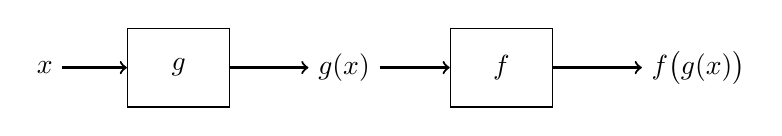
\begin{tikzpicture}[box/.style={draw, minimum width=1.3cm, minimum height=1.0cm}]
  \node (x)   at (0,0)   {$x$};
  \node[box] (g)  at (1.7,0) {$g$};
  \node (gx)  at (3.8,0) {$g(x)$};
  \node[box] (f)  at (5.8,0) {$f$};
  \node (fgx) at (8.3,0) {$f\big(g(x)\big)$};
  \draw[->, thick] (x)--(g);
  \draw[->, thick] (g)--(gx);
  \draw[->, thick] (gx)--(f);
  \draw[->, thick] (f)--(fgx);
\end{tikzpicture}
\end{center}
\noindent Which machine acts \emph{first}, $f$ or $g$? \underline{\hspace{3cm}}

\medskip
\noindent\textbf{D3.\quad Let $f(x)=3x-4$ and $g(x)=2x+2$.}
\begin{enumerate}[itemsep=0.1cm, label=(\alph*)]
  \item Find $f\big(g(x)\big)$ by feeding $g(x)$ into $f$. \vfill
  \item Find $g\big(f(x)\big)$. \vfill
  \item Are they equal? What does this tell you about the order of composition? \vfill
\end{enumerate}

\newpage

%================================================================
%--- Part E: composition + recover the hidden function ---
%================================================================
\noindent\textbf{\large Part E --- Composition and recovering a hidden function}

\medskip
\noindent Read $f\circ g$ as ``$g$ goes first, then $f$ wraps around it'':
$(f\circ g)(x)=f\big(g(x)\big)$. \quad\textbf{$\circ$ is not multiplication.}

\medskip
\noindent\textbf{E1.}\quad The function $f$ is defined by $f(x)=3x-4$, and
$(f\circ g)(x)=6x+2$. Find $g(x)$.

\noindent\emph{The input to $f$ is now $g(x)$, so $f\big(g(x)\big)=3\,g(x)-4$. Set this
equal to $6x+2$ and solve for $g(x)$.}
\vfill

\noindent\textbf{E2.}\quad The function $f$ is defined by $f(x)=2x+1$, and
$(f\circ g)(x)=2x+7$. Find $g(x)$.
\vfill

\noindent\textbf{E3.\quad Recover the outer function.}\quad Given $g(x)=x-3$ and
$(f\circ g)(x)=4x-5$, find $f(x)$.

\noindent\emph{Hint: let $u=x-3$, so $x=u+3$; write $f(u)$ in terms of $u$.}
\vfill

\noindent\textbf{E4.\quad Spot the error.}\quad A student claims $g(x)=\dfrac{6x+2}{3x-4}$
in E1. In one sentence, explain why this is wrong.
\vfill

\newpage

%================================================================
%--- Part F: inverse view + the check habit ---
%================================================================
\noindent\textbf{\large Part F --- The inverse view, and always check}

\medskip
\noindent Another way to recover $g$: if $f$ acts on $g(x)$, then $f^{-1}$ \emph{undoes}
$f$ and hands back $g(x)$: \quad $g(x)=f^{-1}\big((f\circ g)(x)\big)$.

\medskip
\noindent\textbf{F1.}\quad For $f(x)=3x-4$ (from E1):
\begin{enumerate}[itemsep=0.1cm, label=(\alph*)]
  \item Find $f^{-1}(x)$. \vfill
  \item Compute $g(x)=f^{-1}(6x+2)$ and confirm it matches your answer to E1. \vfill
\end{enumerate}

\medskip
\noindent\textbf{F2.\quad The check habit.}\quad Verify E1 by substituting your $g$ back:
compute $f\big(g(x)\big)$ and confirm it equals $6x+2$.
\vfill

\noindent\textbf{F3.\quad Why the inverse view matters.}\quad When the outer function is
\emph{not} linear, substitution is awkward but the inverse still works. Given
$f(x)=x^3$ and $(f\circ g)(x)=8x^3$, find $g(x)$.

\noindent\emph{Hint: $f^{-1}(x)=\sqrt[3]{x}$.}
\vfill

\end{document}
